\subsection{Holdout discrimination and model selection}
Logistic regression had the highest mean validation AUC under both selectors (Table~\ref{tab:building-validation-evidence}). Direct CART selection gave mean AUC 0.834 and sensitivity 0.808; RFE--CART gave AUC 0.838 and sensitivity 0.758. Stacking had lower AUC variance but did not improve mean discrimination or sensitivity over logistic regression. The dummy's perfect sensitivity was accompanied by zero specificity.

\begin{table}[tbp]
\centering
\footnotesize
\setlength{\tabcolsep}{4pt}
\caption{Five-seed holdout validation: mean $\pm$ sample variance at threshold 0.5.}
\label{tab:building-validation-evidence}
\begin{tabular}{@{}lrrrr@{}}
\toprule
& \multicolumn{2}{c}{ROC--AUC} & \multicolumn{2}{c}{Sensitivity} \\
\cmidrule(lr){2-3}\cmidrule(l){4-5}
Model & CART & RFE & CART & RFE \\
\midrule
Logistic regression & $\mathbf{0.834 \pm 0.001306}$ & $\mathbf{0.838 \pm 0.001930}$ & $\mathbf{0.808 \pm 0.002257}$ & $\mathbf{0.758 \pm 0.002951}$ \\
Random forest       & $0.798 \pm 0.002135$ & $0.776 \pm 0.001504$ & $0.717 \pm 0.004688$ & $0.717 \pm 0.002083$ \\
XGBoost             & $0.791 \pm 0.001392$ & $0.777 \pm 0.001080$ & $0.742 \pm 0.003819$ & $0.708 \pm 0.000868$ \\
LightGBM            & $0.791 \pm 0.000612$ & $0.772 \pm 0.000973$ & $0.717 \pm 0.006424$ & $0.717 \pm 0.002083$ \\
Stacking            & $0.822 \pm 0.000825$ & $0.812 \pm 0.000558$ & $0.758 \pm 0.005556$ & $0.733 \pm 0.000521$ \\
\midrule
Training-prior dummy& $0.500 \pm 0.000000$ & $0.500 \pm 0.000000$ & $1.000 \pm 0.000000$ & $1.000 \pm 0.000000$ \\
\bottomrule
\end{tabular}
\end{table}
Logistic regression was selected in all five fixed-model comparisons. Direct CART was selected for seeds 42, 21, and 123, and RFE--CART for seeds 7 and 84. The selected procedure's mean internal test AUC was 0.883 (range 0.828--0.915), sensitivity 0.892 (0.792--0.958), specificity 0.708 (0.667--0.792), and F1 0.816 (0.769--0.846). These summaries describe the validation-selected procedure, whose selector varies by seed, rather than a single fixed RFE candidate.

The tuning analysis likewise selected logistic regression in all five seeds. Its selected $C$ values were 0.1, 0.1, 0.1, 1, and 10 in the stated seed order. For seed 42, the best training-CV AUC was 0.8716 for logistic regression, compared with 0.8475 for random forest, 0.8446 for XGBoost, and 0.8485 for LightGBM. These are parameter-search scores, not test estimates.

\subsection{Leave-one-out evaluation}
Logistic regression achieved the highest pooled AUC (0.874), while random forest achieved the highest accuracy (0.799), sensitivity (0.839), and F1 (0.808) among predictive models (Table~\ref{tab:building-lopo-results}). Logistic regression detected 132 of 161 positive records and correctly classified 118 of 158 controls; random forest detected 135 positive records and correctly classified 120 controls. Stacking had the highest specificity (0.772).

\begin{table}[tbp]
\centering
\footnotesize
\caption{Leave-one-out evaluation on 319 held-out predictions per model at threshold 0.5.}
\label{tab:building-lopo-results}
\begin{tabular}{@{}lrrrrrr@{}}
\toprule
Model & Accuracy & ROC--AUC & Sensitivity & Specificity & F1 & FNR \\
\midrule
Logistic regression & 0.784 & \textbf{0.874} & 0.820 & 0.747 & 0.793 & 0.180 \\
Random forest & \textbf{0.799} & 0.857 & \textbf{0.839} & 0.759 & \textbf{0.808} & \textbf{0.161} \\
XGBoost & 0.762 & 0.835 & 0.807 & 0.715 & 0.774 & 0.193 \\
LightGBM & 0.787 & 0.851 & 0.832 & 0.741 & 0.798 & 0.168 \\
Stacking & 0.787 & 0.865 & 0.801 & \textbf{0.772} & 0.791 & 0.199 \\
\midrule
Training-prior dummy & 0.505 & 0.000 & 1.000 & 0.000 & 0.671 & 0.000 \\
\bottomrule
\end{tabular}
\end{table}
The training-prior dummy's pooled AUC of 0.000 is a leave-one-out artefact: excluding a positive record lowers its training prevalence, while excluding a negative record raises it. Its pooled probabilities therefore rank the classes inversely, even though every thresholded prediction is positive. The value is not evidence of useful discrimination.

The two evaluation designs use different training sizes and assessment samples. Higher leave-one-out scores relative to validation therefore cannot be interpreted as an improvement caused by changing the model. The single leave-one-out run supplies no between-seed variance estimate.

\subsection{Effect of reducing the feature count}
Reducing RFE selection from 20 to 10 predictors lowered validation AUC in four of five splits (Table~\ref{tab:iteration-summary}). Mean AUC fell from 0.838 to 0.816, and mean sensitivity from 0.758 to 0.750. Lower between-seed variance did not offset the loss in discrimination, so the 20-feature reference was retained for this comparison. Neither representation achieved mean validation sensitivity of 0.80.

\begin{table}[htbp]
\centering
\footnotesize
\caption{Paired validation comparison. Summary entries are mean $\pm$ sample variance across five seeds, not standard deviation. Bold indicates the higher mean or seed-level value.}
\label{tab:iteration-summary}
\begin{tabular}{lrrrr}
\toprule
& \multicolumn{2}{c}{Validation AUC} & \multicolumn{2}{c}{Sensitivity} \\
Seed & 20 features & 10 features & 20 features & 10 features \\
\midrule
42  & \textbf{0.799} & 0.760 & \textbf{0.792} & \textbf{0.792} \\
7   & \textbf{0.847} & 0.825 & \textbf{0.708} & 0.667 \\
21  & \textbf{0.870} & 0.826 & \textbf{0.833} & 0.750 \\
84  & \textbf{0.887} & 0.856 & \textbf{0.750} & \textbf{0.750} \\
123 & 0.786 & \textbf{0.811} & 0.708 & \textbf{0.792} \\
\midrule
Mean $\pm$ variance &
$\mathbf{0.838}\pm0.001930$ & $0.816\pm0.001223$ &
$\mathbf{0.758}\pm0.002951$ & $0.750\pm0.002604$ \\
\bottomrule
\end{tabular}
\end{table}
\subsection{Predictive associations and recurring errors}
CRP, vitamin D, extracellular-fluid/total-body-water ratio, and haemoglobin were selected in all five RFE logistic fits. Their mean transformed-scale coefficients were $-1.318$, $+0.690$, $+0.810$, and $+0.549$, respectively; corresponding mean validation permutation AUC decreases were 0.1127, 0.0437, 0.0597, and 0.0172. CRP was the root variable in all five direct CART selection trees, although the recorded-scale cut-point varied from 0.585 to 0.79.

\begin{figure}[tbp]
\centering
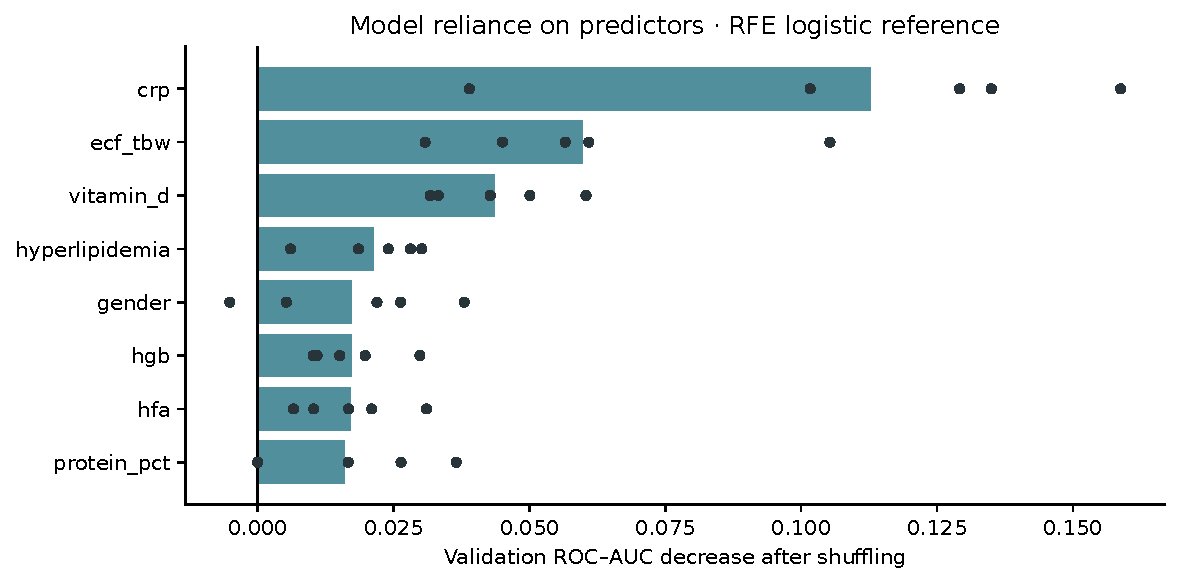
\includegraphics[width=0.9\linewidth]{figures/modeling/permutation_patterns.pdf}
\caption{Validation permutation contributions in the 20-feature RFE logistic reference. Bars show mean AUC decreases; points represent five fitted splits, each averaging 20 shuffles. These values describe model reliance and are not causal effects.}
\label{fig:permutation}
\end{figure}

Source record 117 was a false negative in both appearances among selected-model holdout tests and in four of five predictive leave-one-out models. Records 291 and 316 were false positives in all three of their respective selected-model test appearances and in all five predictive leave-one-out models. These retrospectively selected examples indicate recurring errors across overlapping evaluations, not repeated clinical visits or estimates of future error prevalence.
